\chapter{Dataset}\label{s:ds}

\section{Introduction}\label{s:ds-intro}

As I explained in the Abstract, I chose \modanet after having looked at many others.

An interesting one I found, for example, was DeepFashion \cite{DeepFashion2}, but it didn't feature any footwear annotations unfortunately -- which were the main focus of the task I was given. It had over 800 thousand images though!

\begin{figure}[H]
	\centering
	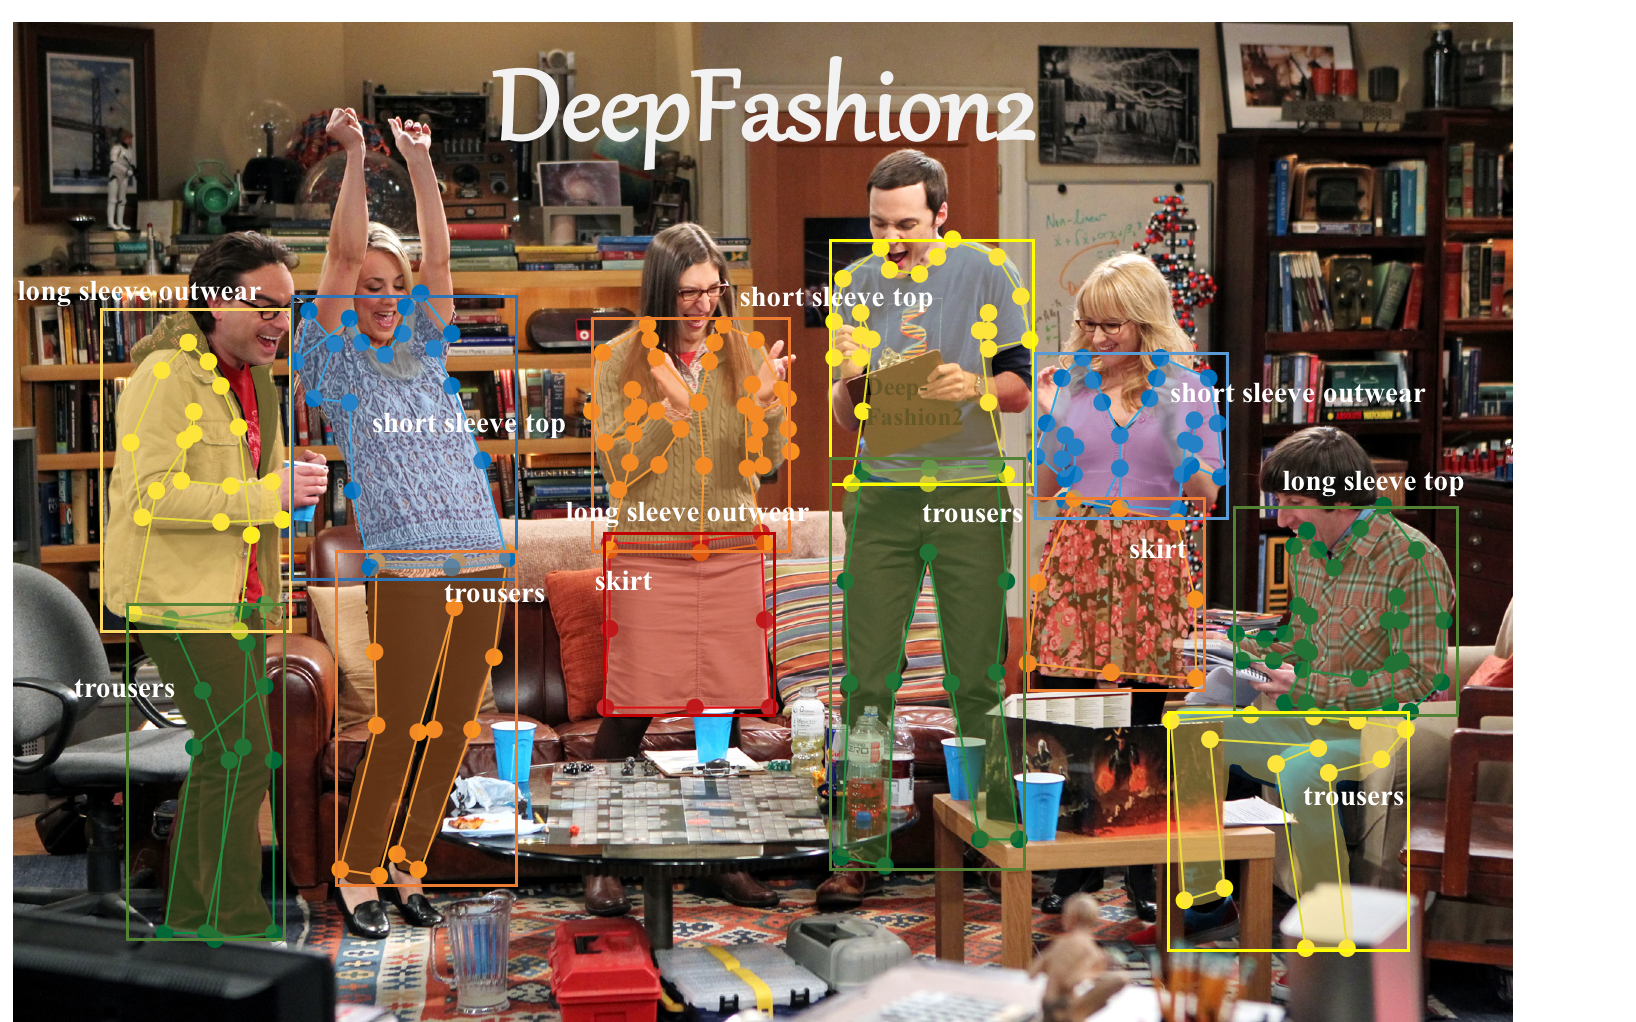
\includegraphics[width=0.75\textwidth]{images/deepfashion2_bigbang}
	\caption{DeepFashion2 feature image.}
	\label{f:deepfashion2_bigbang}
\end{figure}

But what is a dataset? Simply speaking, a dataset is a collection of data that is usually useful for statistics / data analysis purposes. Many datasets today cannot be fully exploited due to our technology, but this is rapidly changing as we continue to develop new algorithms capable to \emph{generalize} better the features that these datasets expose.

For our task, what we needed was a dataset of real-world images that could ideally differenciate between any model, brand and size of any kind of apparel. That means anything you can wear (and buy) could be retrieved by this ideal model, along with the prices when it was bought and the prices now\dots

Unfortunately, one can dream as big as he wants, but the reality is that \modanet is the best I could find, as you can clearly see below in this comparison between competing datasets.

\begin{table}[H]
	\centering
	\caption{Comparison of ModaNet with other datasets for fashion parsing. ModaNet surpasses previous datasets in terms of annotation granularity and scale. \checkmark$^*$  indicates the annotations are not included in the original dataset. The count of categories excludes non-fashion categories, such as \emph{hair}, \emph{skin}, \emph{face}, \emph{background} and \emph{null}.}
	\label{t:datasets}
	\resizebox{\columnwidth}{!}{
	\begin{tabular}{@{}lcccccc@{}}
		\hline
		& DeepFashion~\cite{liu2016deepfashion} & CFPD~\cite{liu2013fashion}    & CCP~\cite{yang2014clothing}     & Fashionista~\cite{yamaguchi2012parsing} & HPW\cite{liang2015deep} & ModaNet~\cite{Zheng_2018}  \\
		\hline
		\# of images      & $800,000$   & $2,682$ & $1,004$ & $685$       & $1,833$ & $55,176$ \\
		\# of categories  &     50        &     19    &      56   &       53      &  11  & 13  \\
		Pixel annotation & \texttimes      & \checkmark    &\checkmark & \checkmark      &\checkmark & \checkmark      \\
		Bounding box      & landmarks   &  \checkmark$^*$       & \checkmark$^*$         &     \checkmark$^*$         & \checkmark$^*$  & \checkmark      \\
		Polygon           & \texttimes        & \texttimes     & \texttimes     & \texttimes        &\texttimes  & \checkmark      \\ 
		\hline
	\end{tabular}
	}
\end{table}

Then I stumbled upon this great dataset. It had much richer annotations, with \emph{almost-perfect} and very precise masks for each instance, plus it included footwear too!
\modanet has been annotated and managed by eBay researchers.
Here is their brief description of their work (on their GitHub page):
\begin{quotation}
	ModaNet is a street fashion images dataset consisting of annotations related to RGB images. ModaNet provides multiple polygon annotations for each image. This dataset is described in a technical paper with the title \emph{ModaNet: A Large-Scale Street Fashion Dataset with Polygon Annotations} \cite{zheng/2018acmmm}. Each polygon is associated with a label from 13 meta fashion categories. The annotations are based on images in the PaperDoll image set, which has only a few hundred images annotated by the superpixel-based tool. The contribution of ModaNet is to provide new and extra polygon annotations for the images.
\end{quotation}


\section{PaperDoll}\label{s:ds-paperdoll}

The PaperDoll dataset \cite{yamaguchi2013paper} is an expansion of the Fashionista dataset \cite{yamaguchi2012parsing}, which were all developed without deep learning in mind. In fact, they initially used HOGs, cited briefly in \sref{s:nnevo-intro}. They only managed to do \emph{Semantic Segmentation} [\sref{s:patt-sema}] though.

\begin{figure}[H]
	\centering
	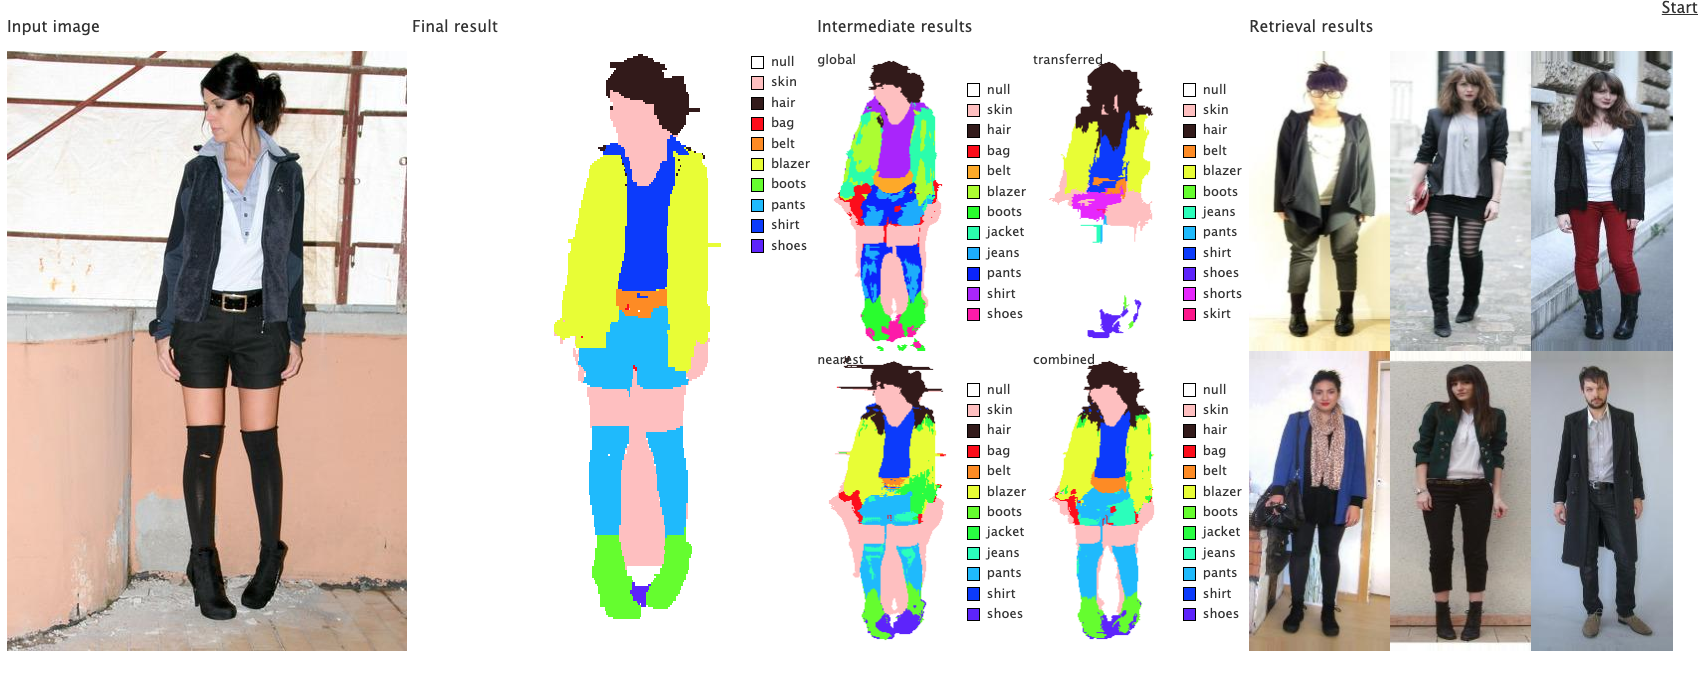
\includegraphics[width=\linewidth]{images/paperdollparsing}
	\caption{Results of the PaperDoll parsing from 2013, still online at \texttt{clothingparsing.com}}
	\label{f:paperdollparsing}
\end{figure}

An interesting thing the PaperDoll dataset added was retrieving related images. In their paper, they acknowledge that many people living in the same environment (i.e. college) also dress in a similar style.

They achieved this with a method that gave the name to the dataset: 
“like laying paper cutouts of clothing items onto a paper doll", each query generates related images that are subsequently fed back to the query to enlarge the database annotation.

\begin{figure}[H]
	\centering
	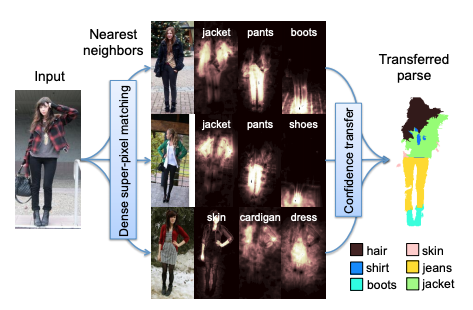
\includegraphics[width=.75\linewidth]{images/paperdolltransfer}
	\caption{Transferred parse. Likelihoods in nearest neighbors are transferred to the input via dense matching.}
	\label{f:paperdolltransfer}
\end{figure}

\subsection{The source: Chictopia}\label{s:ds-paperdoll-chictopia}

\texttt{chictopia.com} is a social network focused on fashion.
The data from the site was not available until January \nth{31}, 2019. It was crawled originally in Fall 2012.
That is the date when, thanks to the new copyright law in Japan \footnote{European Alliance for Research Exellence, September \nth{3}, 2018: \emph{Japan amends its copyright legislation to meet future demands in AI and big data}}  , the researchers decided to release the raw dataset for research purposes.

Thanks to this we can enjoy training our algorithms on the raw paperdoll data annotated with \modanet.

\subsection{The RAW Data}\label{s:ds-paperdoll-raw}

The raw data is available on the paperdoll GitHub repo, along with the instructions to download the images.
The dataset requires SQLite3 and LMDB. After you download the ~40GB database file, you have to extract it and then the images are encapsulated in the database with some labels (not anywhere rich as the ModaNet ones, nor in the COCO format ready to be trained).
For example, you could retrieve all the photos taken by a particulare chictopia user (not very useful). Or you could use the post tag relationships, which I have not used—but they could become very useful for future work!

Here are the post tag relationships, retrievable in SQL style:
\begin{itemize}
	\item Color: color of the item.
	\item Style: general style of the post.
	\item Occasion: occasion of the outfit.
	\item Clothing: type of the item.
	\item Brand: brand of the item.
	\item Trend: free-form tag.
\end{itemize}

I think in particular, \emph{Brand} is definitely the most interesting one, especially because of the original intent of this thesis, explained in the Introduction. The \emph{Occasion} could also be useful in determining where an item is worn.

There are also relationships between users. A user has many friends and fans, so in theory you could track how well a \emph{Creator}, which in italy are called \emph{Influencers}, has been “selling" the items he or she is sponsoring!

All it's needed is to integrate the \modanet annotations with the sparse information on the paperdoll SQL database and add a dataset comprising of the specific models of each clothing and apparel item. (this sounds too simple I know)

More on that on \sref{s:conclusion}

\section{ModaNet}\label{s:ds-modanet}

\begin{quotation}
	“Clothing recognition is a challenging and societally important problem – global sales for clothing total over a hundred billion dollars, much of which is conducted online." \cite{yamaguchi2013paper}
\end{quotation}

\begin{table}[H]
\centering
\small
\caption{\textbf{ModaNet labels}. Meta categories are groups of highly related raw categories}
\label{t:modanet statistics}
\begin{tabularx}{\textwidth}{@{}lXccc@{}}
\hline
Meta & Raw & \#Train & \#Val & Avg Inst. size\\
\hline
bag  & bag & $36,699$  & $2,155$  & 4.88\% \\
belt  & belt & $13,743$ & $771$ & 0.46\% \\
boots  & boots & $7,068$ & $691$ & 2.40\%  \\
footwear  & footwear & $39,364$ & $1,617$ & 0.96\% \\
outer  & coat, jacket, suit, blazers
%, cardigan, sweater, jumpsuits, rompers, vest 
& $23,743$ & $1,358$ & 7.48\% \\
dress  & dress, t-shirt dress & $14,460$ & $804$ & 10.49\% \\
sunglasses  & sunglasses &  $8,780$ & $524$ & 0.31\% \\
pants  & pants, jeans, leggings & $23,075$  &  $1,172$ & 5.65\% \\
top  & top, blouse, t-shirt, shirt & $34,745$ & $1,862$ & 4.83\% \\ 
shorts  & shorts & $5,775$ & $429$ & 2.86\% \\ 
skirt  & skirt & $10,860$  & $555$ &  6.40\% \\ 
headwear  & headwear & $5,405$ & $491$ & 1.25\% \\ 
scarf\&tie  & scarf, tie & $3,990$ & $378$ & 2.55\%  \\ 
\hline
\end{tabularx}
\end{table}

As said above at the end of \sref{s:ds-intro}, \modanet provides high quality annotations to $\sim$50k images on the PaperDoll dataset. The annotations include masks, bounding boxes and categories (label). The labels are defined above in \tref{t:modanet statistics}.

The rich annotation of the dataset allows to measure the performance of state-of-the-art algorithms for instance segmentation.

These annotations include images with many pose variations, using polygons for segmentation. In this way, training on this data grants a more generalizable model.

\subsection{How ModaNet was constructed}\label{s:ds-modanet-constr}

They collected 1 million images from the PaperDoll dataset, then they applied Faster R-CNN \cite{ren2015faster} pretrained on COCO dataset \sref{s:coco} to only select the images with only one person in the image.

From this initial set, they selected 4000 images and divided them in half manually based on their quality and suitability to be annotated. On those images, they set up a classifier for image quality using a model pretrained on ImageNet \sref{s:imagenet} , fine-tuned only on the last layer of a ResNet50 \sref{s:imagenet-resnet}. They applied this classifier to the entire set of images.

Selecting only the high quality (for annotating purposes) images, containing only one person, they had a robust starting point to send over to the human annotators.

The tasks the human annotators had were two: to skip images they think are ambiguous to annotate and to correctly label with polygon annotations each image.

There were 17 annotators (9 female and 8 male).

Let's say an image is dark or blurred in a certain area, that is not a good input for an algorithm to learn from, since the patterns are obscured by these adverse conditions and only confuse the pattern recognition methods.


\subsection{ModaNet structure}\label{s:ds-modanet-struct}

The \modanet structure is of a .json array, frequently used to store results in Python.

\begin{lstlisting}[language=Python]
	{
	'info' : info, 'images' : [image], 'annotations' : [annotation], 'licenses' : [license],
	'year': year, 'categories': [category], 'type': type
	}
	
	info{
	'version' : str, 'description' : str, 'contributor' : str, 'date_created' : datetime,
	}
	
	image{
	'id' : int, 'width' : int, 'height' : int, 'file_name' : str, 'license' : int
	}
	
	license{
	'id' : int, 'name' : str, 'url' : str,
	}
	
	annotation{
	'area': int, 
	'bbox': [x,y,width,height],
	'segmentation': [polygon],
	'image_id': int,
	'id': int,
	'category_id': int,
	'iscrowd': int
	}
	category{
	'supercategory': str, 'id': int, 'name': str,
	}
\end{lstlisting}

It follows the COCO [\sref{s:coco}] dataset competition guidelines.

\subsection{ModaNet results}\label{s:ds-modanet-rs}

% --- figure begins ---%
\begin{figure}[H]
	\centering
	\setlength{\tabcolsep}{0.1pt}
	\setlength{\fboxsep}{0pt}%
	\setlength{\fboxrule}{0.1pt}%
	\renewcommand{\arraystretch}{0.6}
	\begin{tabular}{cccccccccc}
		%\multicolumn{1}{c}{Query} & &\multicolumn{5}{c}{Retrieved Images} & &\multicolumn{1}{c}{Query}  & &\multicolumn{5}{c}{Retrieved Images} & &\multicolumn{1}{c}{Query}  & &\multicolumn{5}{c}{Retrieved Images}\\ 
		%1st row----------------------------
		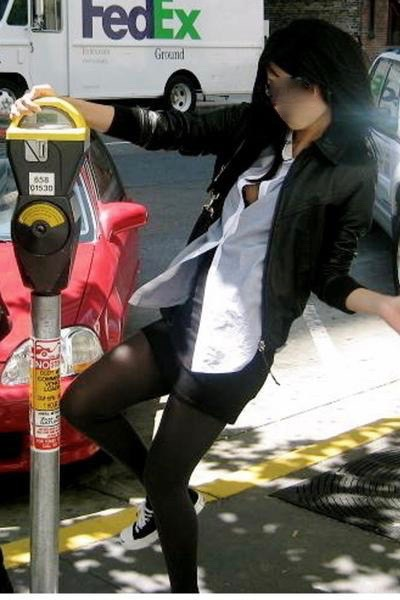
\includegraphics[width=.1\textwidth]{./figures/dataset/0023328_b.jpg} & 
		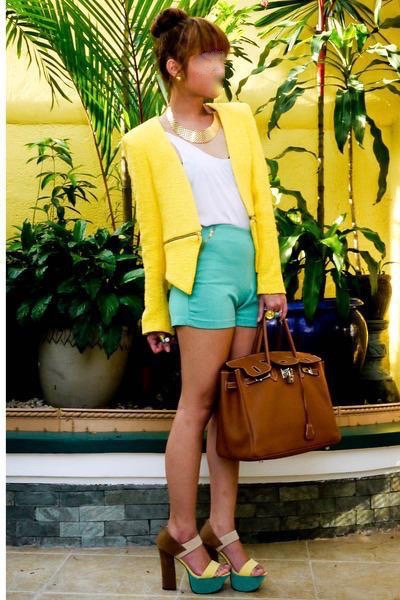
\includegraphics[width=.1\textwidth]{./figures/dataset/0019351_b.jpg} &
		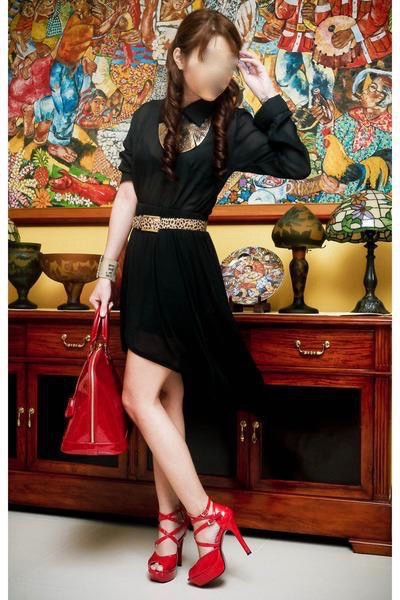
\includegraphics[width=.1\textwidth]{./figures/dataset/0019891_b.jpg} &
		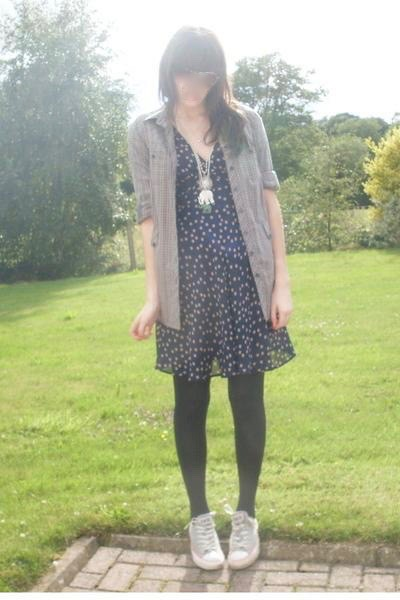
\includegraphics[width=.1\textwidth]{./figures/dataset/0020171_b.jpg} &
		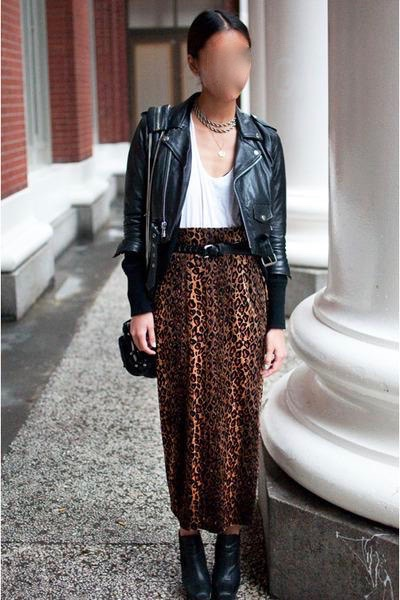
\includegraphics[width=.1\textwidth]{./figures/dataset/0020348_b.jpg} & 
		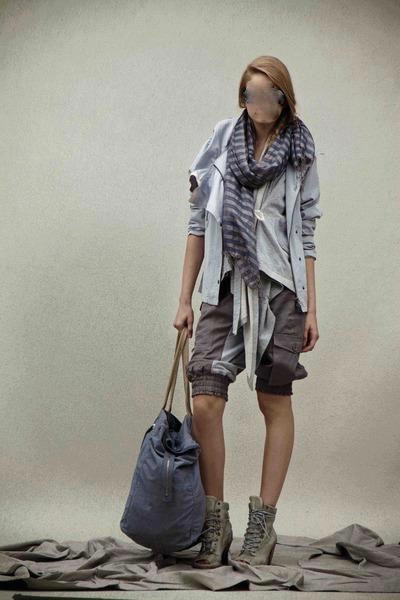
\includegraphics[width=.1\textwidth]{./figures/dataset/0020830_b.jpg} &
		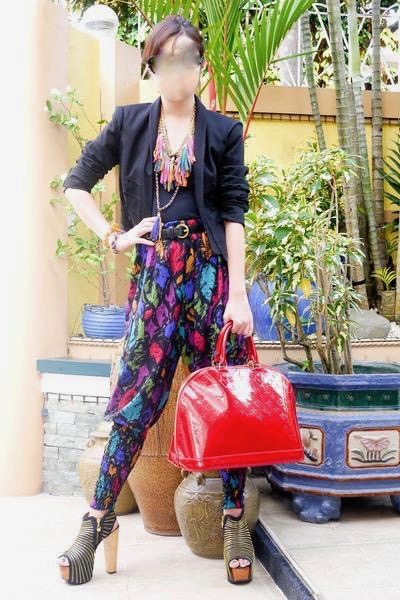
\includegraphics[width=.1\textwidth]{./figures/dataset/0020879_b.jpg} &
		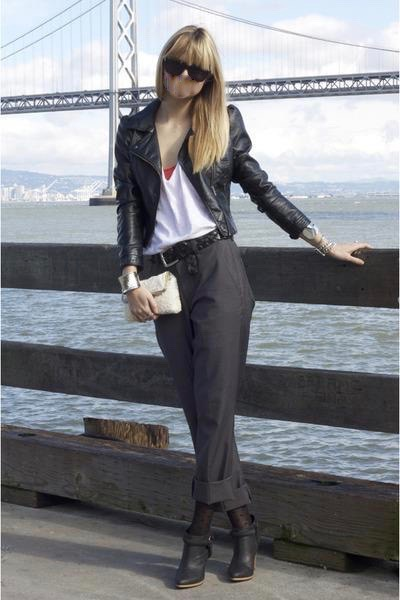
\includegraphics[width=.1\textwidth]{./figures/dataset/0020910_b.jpg} &
		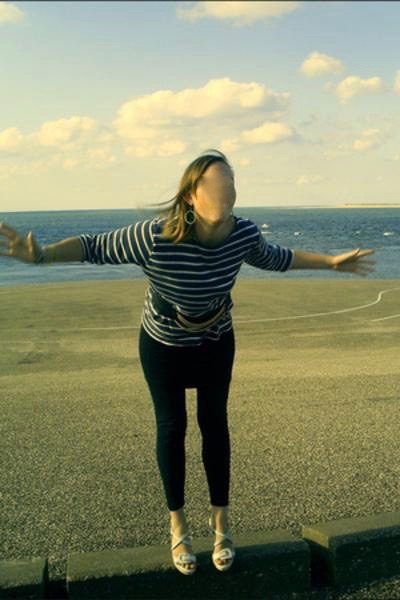
\includegraphics[width=.1\textwidth]{./figures/dataset/0021450_b.jpg} &
		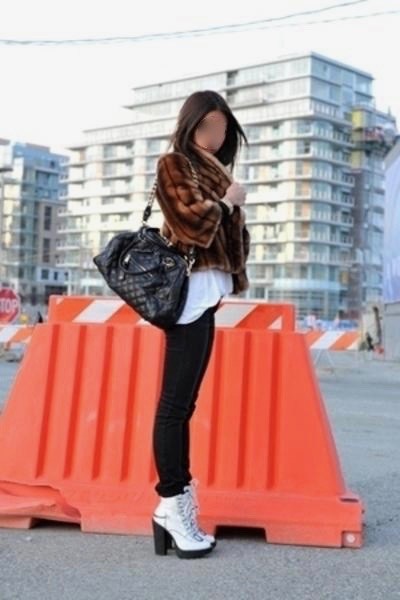
\includegraphics[width=.1\textwidth]{./figures/dataset/0022212_b.jpg}\\
		%\vspace{-5mm}
		%2nd row----------------------------
		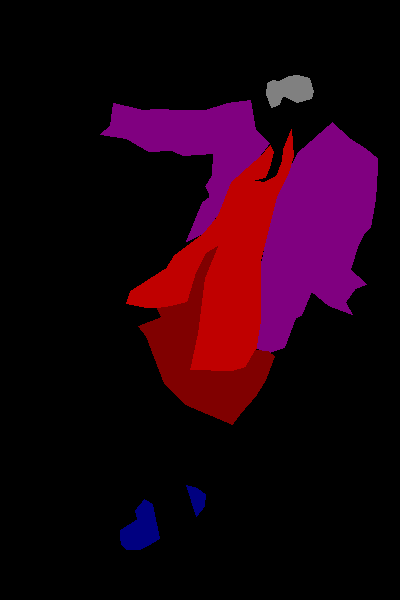
\includegraphics[width=.1\textwidth]{./figures/dataset/0023328.png} & 
		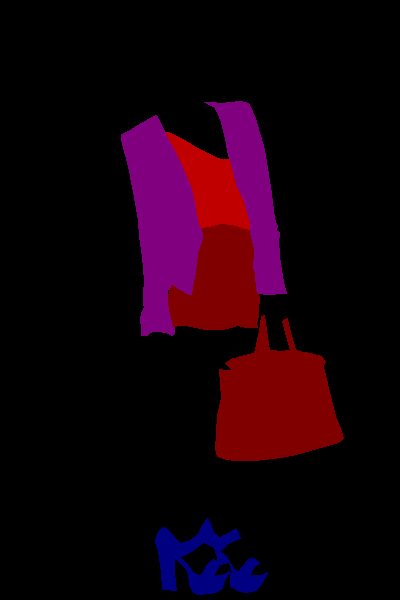
\includegraphics[width=.1\textwidth]{./figures/dataset/0019351.png} &
		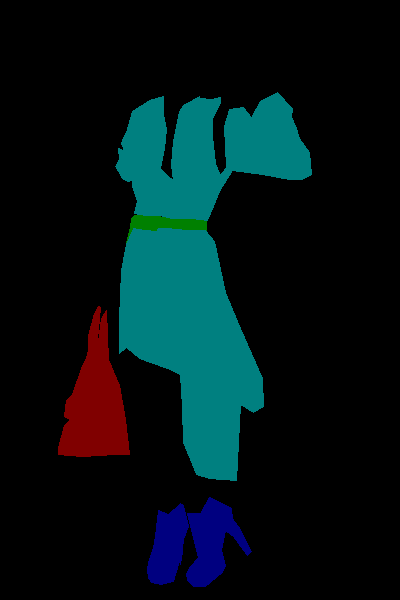
\includegraphics[width=.1\textwidth]{./figures/dataset/0019891.png} &
		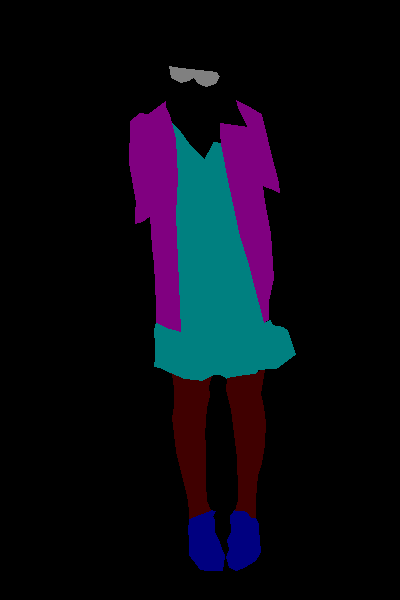
\includegraphics[width=.1\textwidth]{./figures/dataset/0020171.png} &
		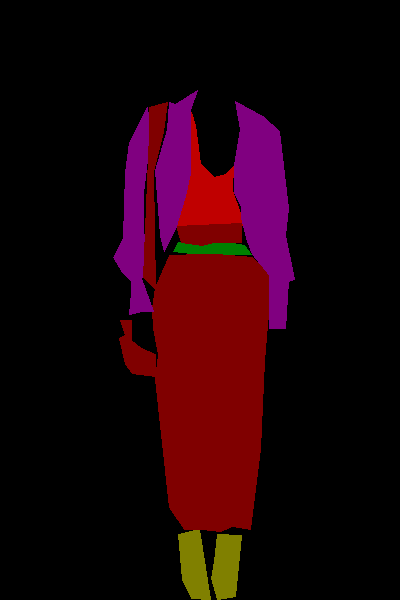
\includegraphics[width=.1\textwidth]{./figures/dataset/0020348.png} & 
		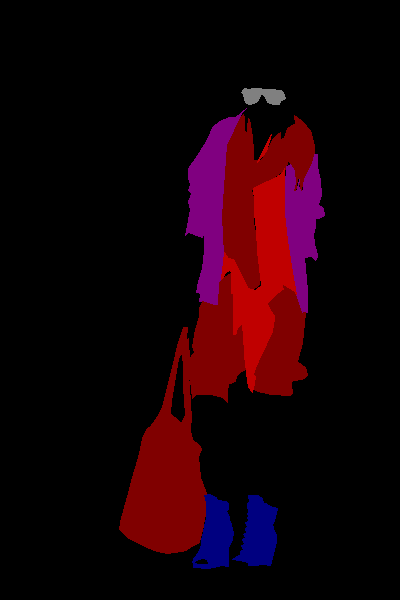
\includegraphics[width=.1\textwidth]{./figures/dataset/0020830.png} &
		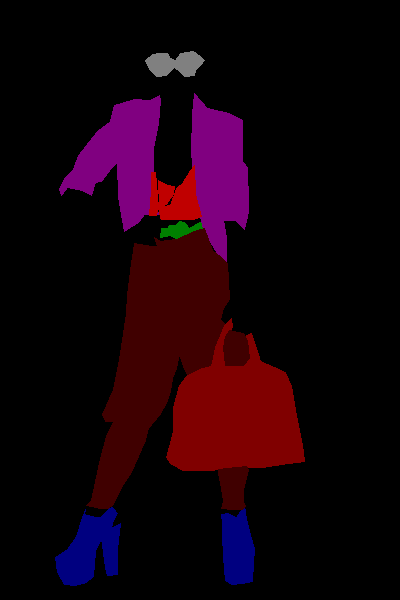
\includegraphics[width=.1\textwidth]{./figures/dataset/0020879.png} &
		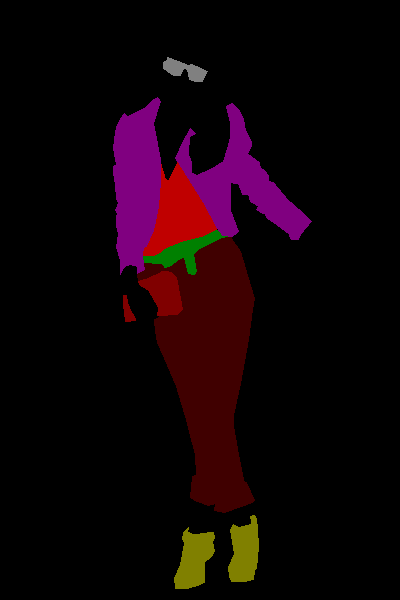
\includegraphics[width=.1\textwidth]{./figures/dataset/0020910.png} &
		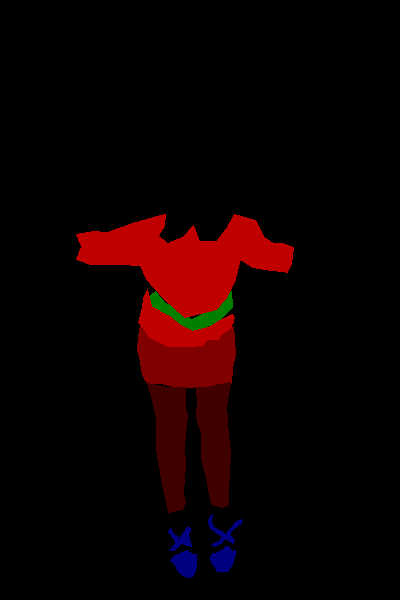
\includegraphics[width=.1\textwidth]{./figures/dataset/0021450.png} &
		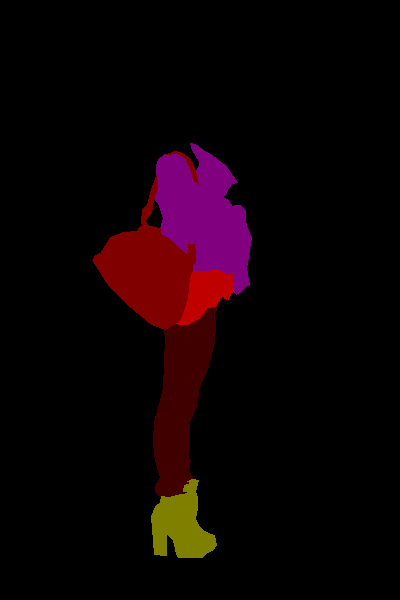
\includegraphics[width=.1\textwidth]{./figures/dataset/0022212.png}\\
		%\vspace{-5mm}
		%3rd row----------------------------
		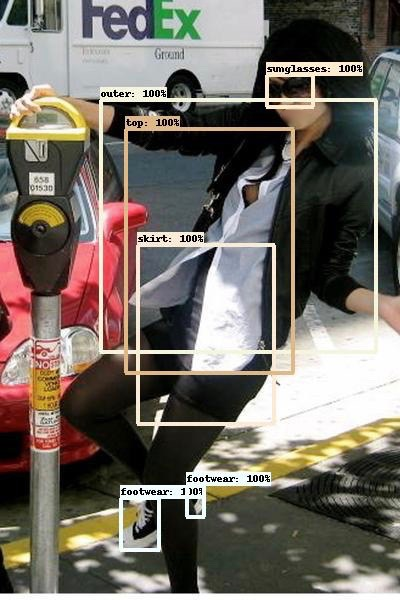
\includegraphics[width=.1\textwidth]{./figures/dataset/0023328_0_5_gt_b.jpg} & 
		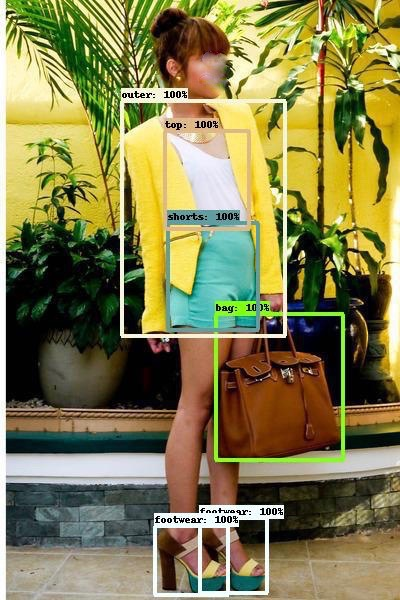
\includegraphics[width=.1\textwidth]{./figures/dataset/0019351_0_5_gt_b.jpg} &
		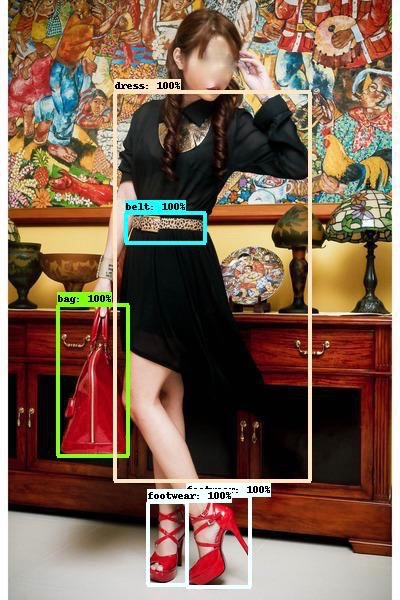
\includegraphics[width=.1\textwidth]{./figures/dataset/0019891_0_5_gt_b.jpg} &
		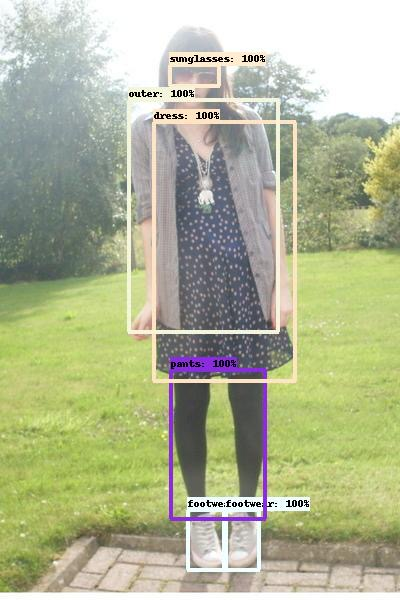
\includegraphics[width=.1\textwidth]{./figures/dataset/0020171_0_5_gt_b.jpg} &
		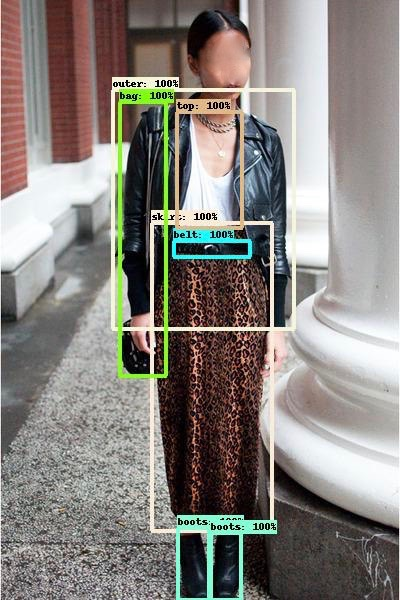
\includegraphics[width=.1\textwidth]{./figures/dataset/0020348_0_5_gt_b.jpg} & 
		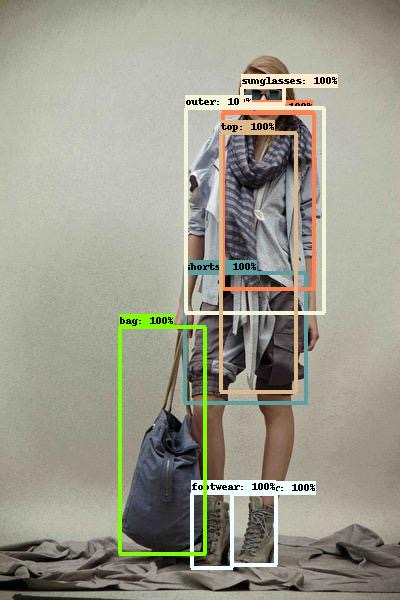
\includegraphics[width=.1\textwidth]{./figures/dataset/0020830_0_5_gt_b.jpg} &
		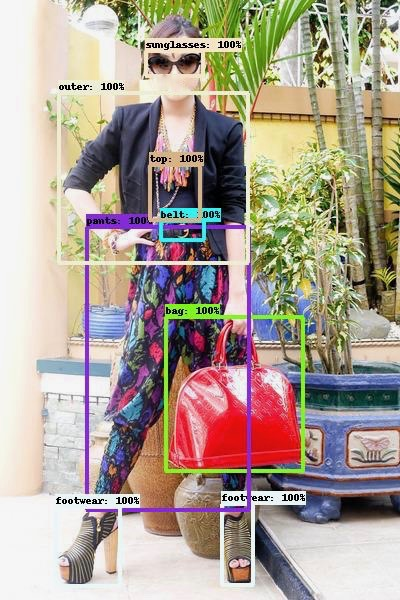
\includegraphics[width=.1\textwidth]{./figures/dataset/0020879_0_5_gt_b.jpg} &
		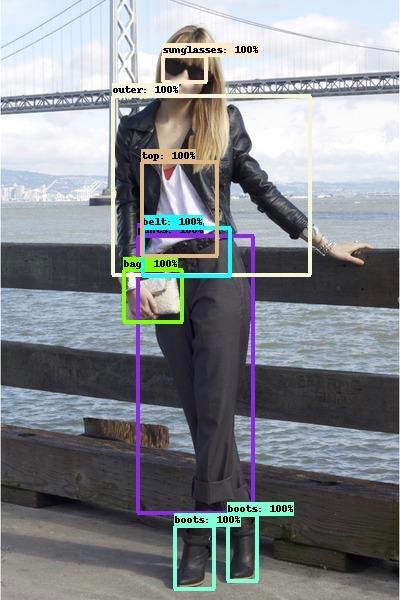
\includegraphics[width=.1\textwidth]{./figures/dataset/0020910_0_5_gt_b.jpg} &
		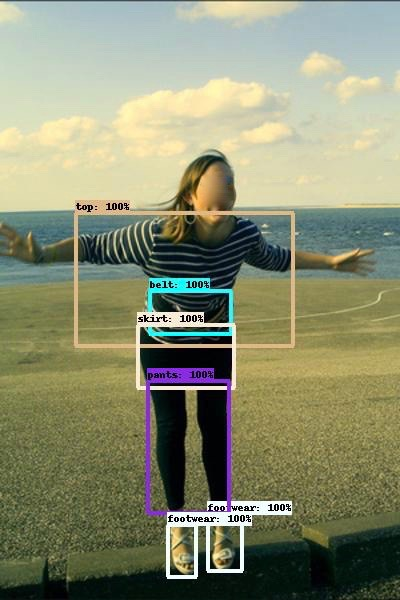
\includegraphics[width=.1\textwidth]{./figures/dataset/0021450_0_5_gt_b.jpg} &
		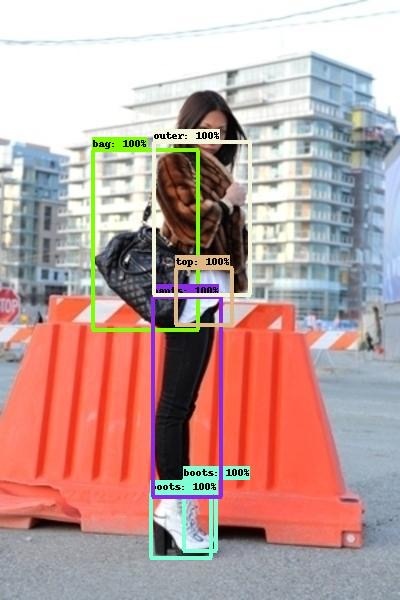
\includegraphics[width=.1\textwidth]{./figures/dataset/0022212_0_5_gt_b.jpg}\\
		
	\end{tabular}
	\caption{Examples of original images with corresponding pixel-level segmentation masks and bounding box annotations of the proposed ModaNet dataset. The first row shows the original color street image containing a person with fashion products. The second row indicates the pixel-wise annotation for the fashion product, where color is encoded to represent the fashion product category. The third row represents the bounding box annotation overlaying on the color images.}
	\label{fig:annotations} %% label for entire figure
\end{figure}
% --- figure ends --- % 



\begin{figure}[H]
	\begin{center}
		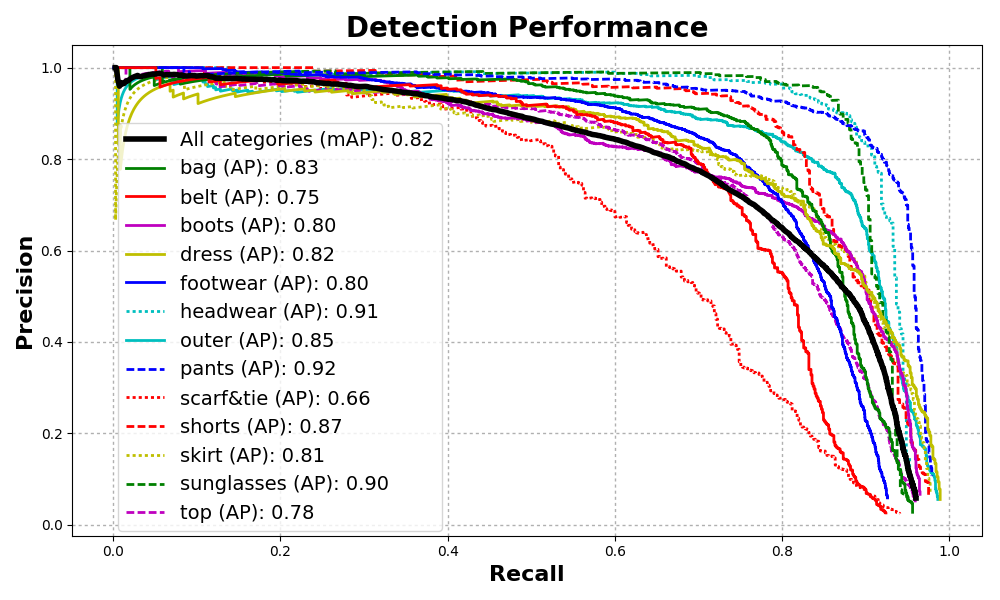
\includegraphics[width=.32\linewidth]{./figures/faster_pr_0_5.png}
		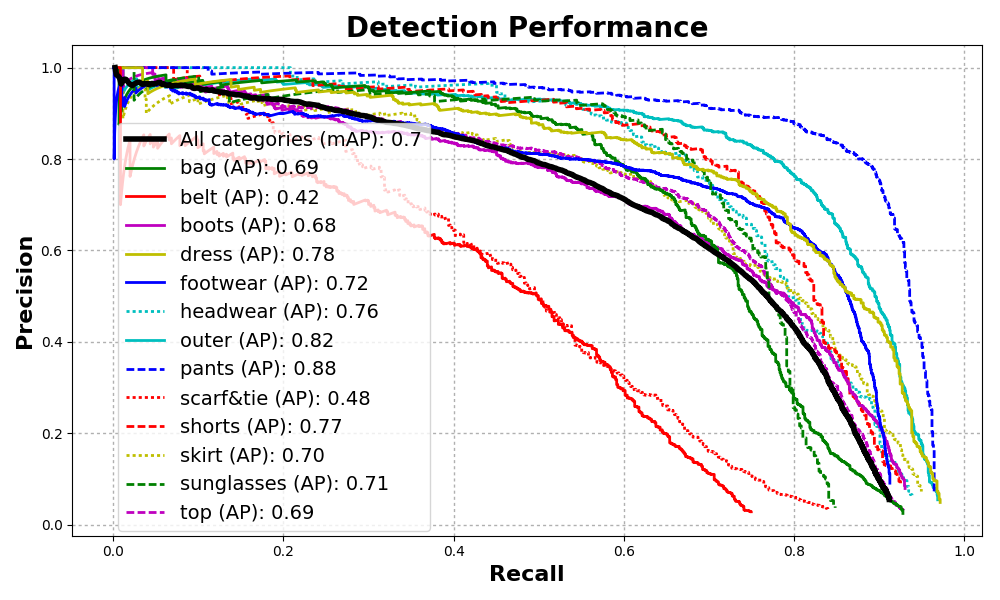
\includegraphics[width=.32\linewidth]{./figures/ssd_pr_0_5.png}
		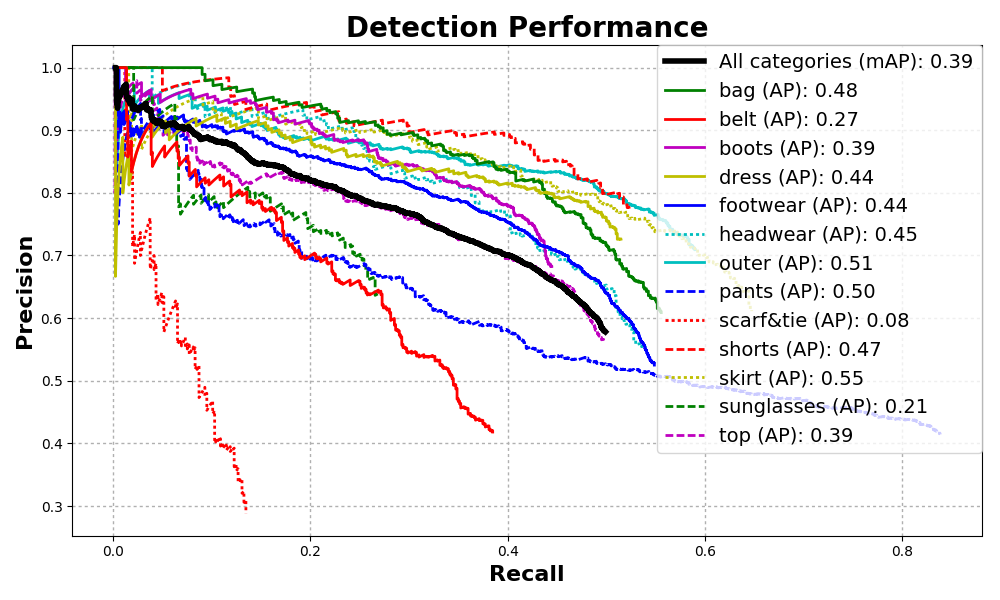
\includegraphics[width=.32\linewidth]{./figures/yolo_pr_0_5.png}
	\end{center}
	\vspace{-2mm}
	\caption{Performance comparison of Faster RCNN (left), SSD (middle) and YOLO (right).}
	\label{fig:map-per-cat}
\end{figure}

% --- figure begins ---%
\begin{figure}[H]
	\centering
	\setlength{\tabcolsep}{0.5pt}
	\setlength{\fboxsep}{0pt}%
	\setlength{\fboxrule}{0.1pt}%
	\renewcommand{\arraystretch}{0.6}
	\begin{tabular}{cccc}
		%\multicolumn{1}{c}{Query} & &\multicolumn{5}{c}{Retrieved Images} & &\multicolumn{1}{c}{Query}  & &\multicolumn{5}{c}{Retrieved Images} & &\multicolumn{1}{c}{Query}  & &\multicolumn{5}{c}{Retrieved Images}\\ 
		%1st row----------------------------
		GT & Faster RCNN & SSD & YOLO \\
		%2nd row----------------------------
		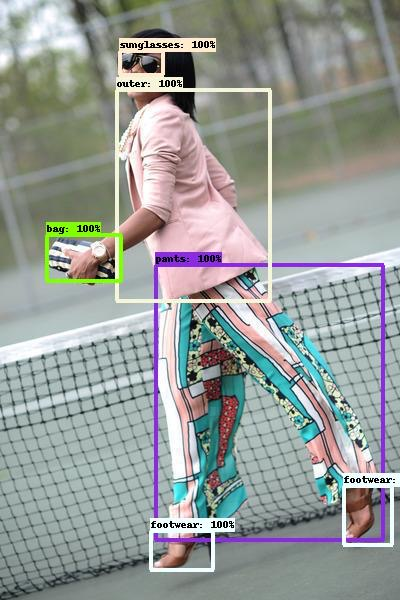
\includegraphics[width=.11\textwidth]{./figures/detection/0111624_0_5_gt_b.jpg} & 
		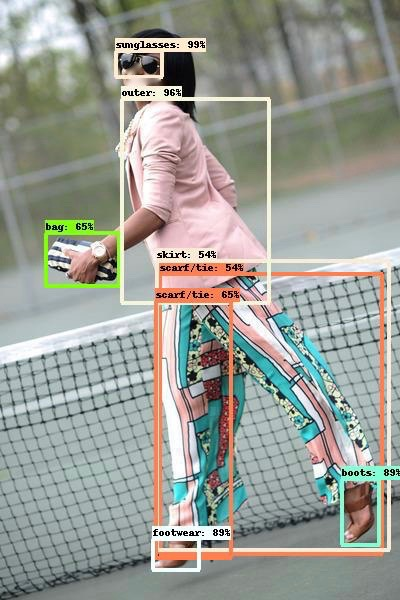
\includegraphics[width=.11\textwidth]{./figures/detection/faster_0111624_0_5_det_b.jpg} &
		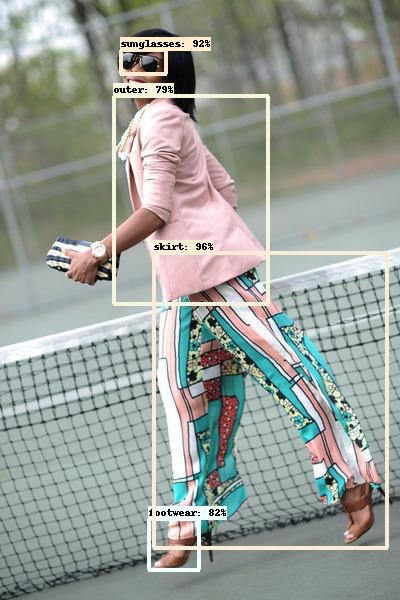
\includegraphics[width=.11\textwidth]{./figures/detection/ssd_0111624_0_5_det_b.jpg} &
		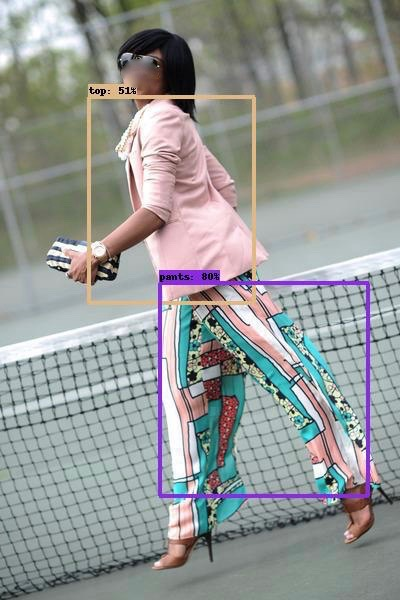
\includegraphics[width=.11\textwidth]{./figures/detection/yolo_0111624_0_5_det_b.jpg}\\
		
		%3rd row----------------------------
		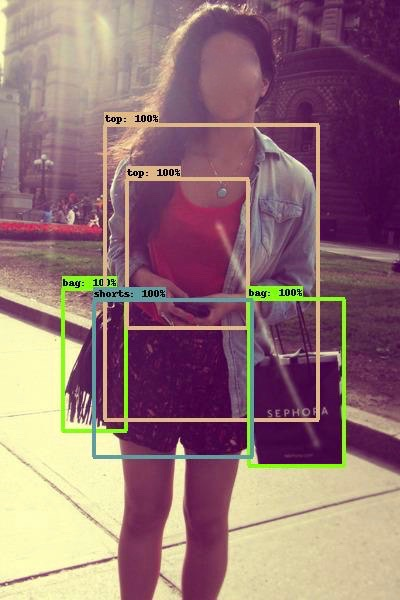
\includegraphics[width=.11\textwidth]{./figures/detection/0120462_0_5_gt_b.jpg} & 
		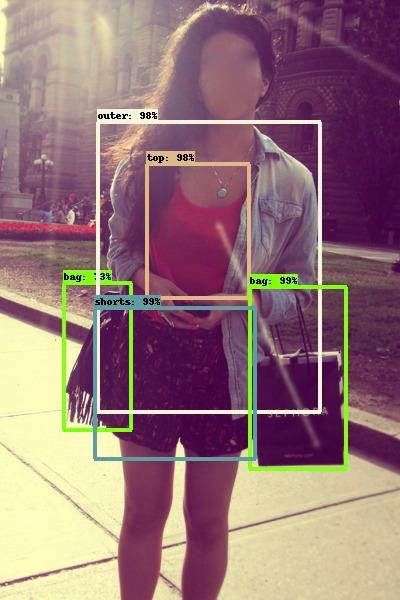
\includegraphics[width=.11\textwidth]{./figures/detection/faster_0120462_0_5_det_b.jpg} &
		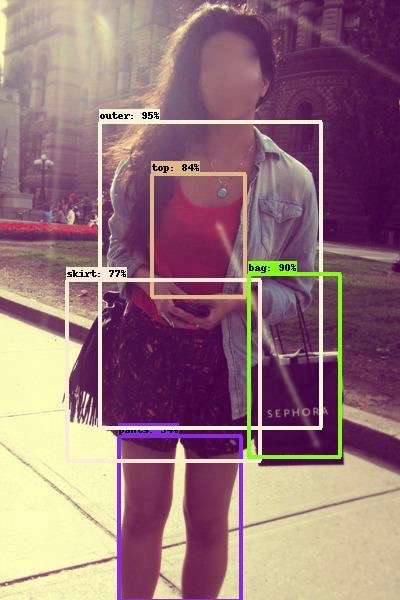
\includegraphics[width=.11\textwidth]{./figures/detection/ssd_0120462_0_5_det_b.jpg} &
		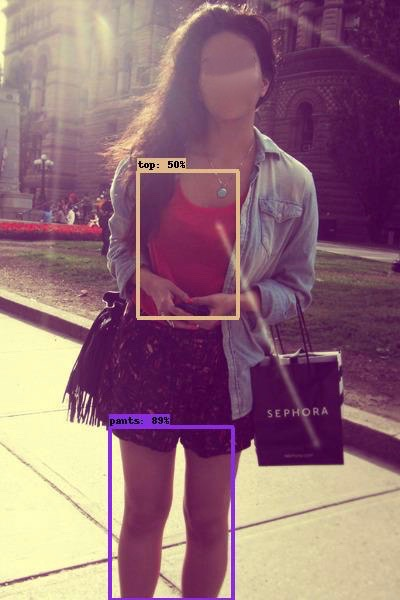
\includegraphics[width=.11\textwidth]{./figures/detection/yolo_0120462_0_5_det_b.jpg}\\
		
		%4th row----------------------------
		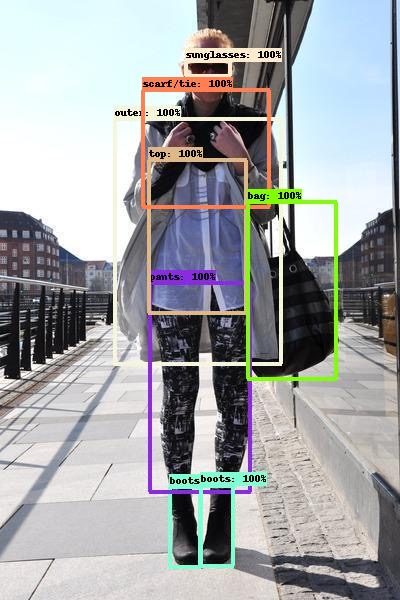
\includegraphics[width=.11\textwidth]{./figures/detection/0124208_0_5_gt_b.jpg} & 
		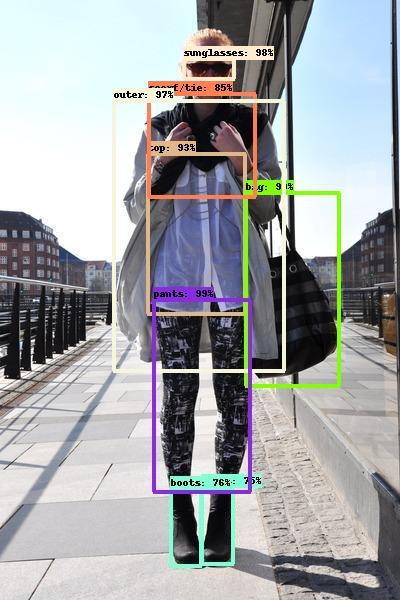
\includegraphics[width=.11\textwidth]{./figures/detection/faster_0124208_0_5_det_b.jpg} &
		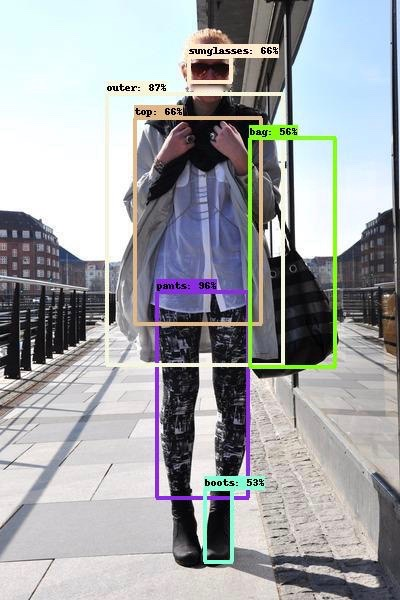
\includegraphics[width=.11\textwidth]{./figures/detection/ssd_0124208_0_5_det_b.jpg} &
		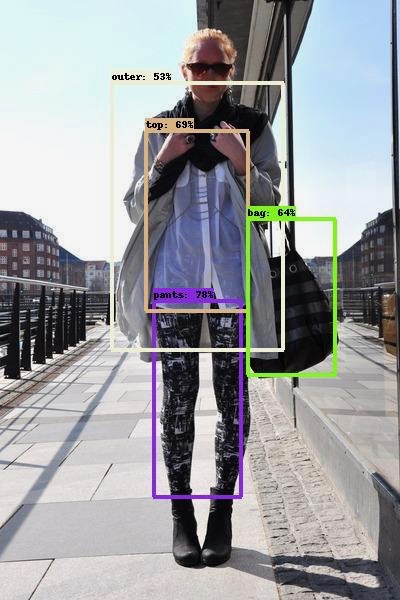
\includegraphics[width=.11\textwidth]{./figures/detection/yolo_0124208_0_5_det_b.jpg}\\
	\end{tabular}
	\caption{Qualitative comparisons of Faster RCNN, SSD and YOLO.}
	\label{fig:detection-qual} %% label for entire figure
\end{figure}
% --- figure ends --- % 

\section{Organizing the Dataset}\label{s:ds-org}

Organizing the dataset has been an enourmous feat, at least for a newbie like me.

First I had to download PaperDoll, about 40GB size. Then ModaNet.

The structure I ended up with looks like this:

\begin{figure}[H]
	\centering
	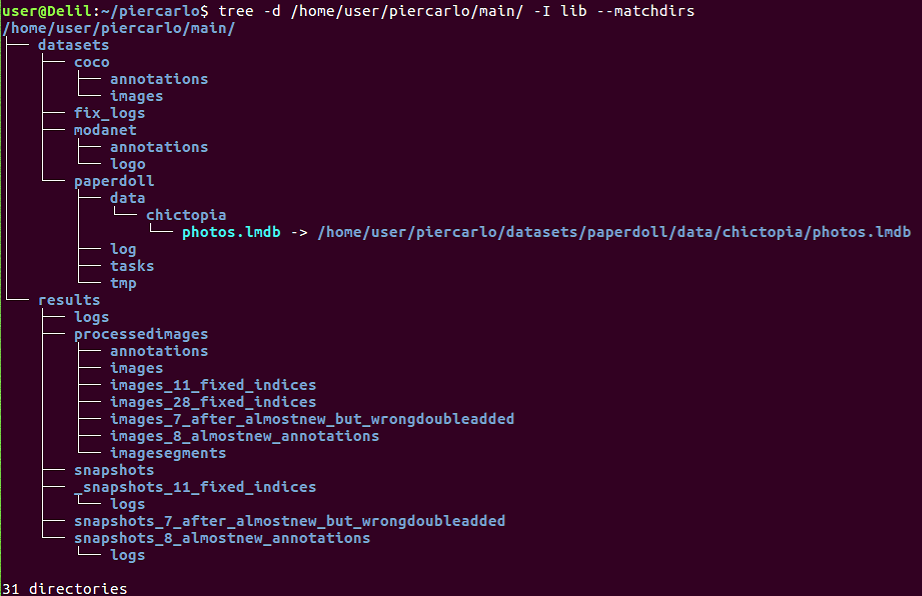
\includegraphics[width=\linewidth]{images/datastructure}
	\caption{Final data structure produced by my package (and used also before creating it)}
	\label{f:datastructure}
\end{figure}


\subsection{Organizing PaperDoll}\label{s:ds-org-pd}

The PaperDoll dataset came into a compressed (.tar) SQL format. That is great for only extracting the images you want, not so great if you just want to download them all easily. The data structure of the SQL database is explained in \sref{s:ds-paperdoll-raw}.

\begin{lstlisting}[language=bash]
$ wget http://vision.is.tohoku.ac.jp/chictopia2/photos.lmdb.tar
$ tar xf photos.lmdb.tar
$ gunzip -c chictopia.sql.gz | sqlite3 chictopia.sqlite3
\end{lstlisting}


This below is -- in short, and omitting the class used to handle the PhotoData -- the code I developed to extract the files from the database. It is available in my GitHub repo, \emph{github.com/cad0p/maskrcnn-modanet} under the file arrange\_images.py

\lstinputlisting[language=Python, firstline=43, lastline=68]{../maskrcnn-modanet/maskrcnn_modanet/arrange_images.py}
% if this doesn't load, clone the maskrcnn-modanet repo in the same main folder (mine is called GitHub) 

% if it is not aligned, just roll back to v1.0.1 and it will be all aligned.

So basically I opened the ModaNet annotations and looked for the images that are used in the annotations (about 50 thousand). Those are the \emph{instances} dictionary, that has the same structure as the one explained above in \sref{s:ds-modanet-struct}.

That high number you see is the max id on the dataset. 

To debug, I was advised by Leonardo to use \emph{ipdb}, a nice debugger that you see commented in the code, that lets you see what happens step by step.

The SQL string I formatted contains all the images ids in the annotations, so if the image is in the annotations, it will be extracted.

\lstinputlisting[language=Python, firstline=96, lastline=105]{../maskrcnn-modanet/maskrcnn_modanet/arrange_images.py}

Here I use the aforementioned PhotoData class to get the raw image file and save it to the desired img\_path location.

\subsection{Organizing ModaNet}\label{s:ds-org-mn}

Organizing \modanet has been simpler, meaning that the .json file containing the annotations was readily available, although I quickly discovered that what they called the “train" dataset was actually the whole annotations, and the “val" ones were only annotated with bboxes and only served the purpose of being a reference for a competition (that doesn't interest us since it's only for object detection algorithms).

So I simply moved the train annotations into the instances\_all.json file under datasets/coco/annotations and then the real work started: splitting the annotations into training, validation and test set. I didn't really use the test set, but it may become useful in later developements.

The training set consists of the images the algorithm uses to learn the features of the objects [by adjusting the loss function, \sref{s:losses}]. 
The validation set serves as a way to evaluate the work the algorithm has been doing (and those annotations are never seen by the algorithm during training). The evaluation is done with AP and AR metrics at various IoUs, described in \sref{s:trainalg-evalmetrics}. The evaluation can also be qualitatively by looking at examples from the validation set (or the test set, depending on the use case).

The work of splitting the annotations is described in \sref{s:splitting}, under the \emph{Training Strategies} chapter, because it's a training strategy decision. However, we can say here that the annotations must be split as evenly as possible regarding the number of annotations of one type vs. another, so that they contain as similar of a composition as possible. Just like for exit polls in the elections, or any reasonably done survey, they have to try have the most balanced mix of responders.

\subsubsection{The Fix.}\label{s:ds-mn-fix}

At the end of my work at IMP Lab, I discovered that the reason why the algorithm wasn't picking up well on footwear and boots was because most annotations had the bounding boxes overlapped, just like for the image below: (0892135.jpg is the source file)

% --- figure begins ---%
\begin{figure}[H]
	\centering
	\setlength{\tabcolsep}{0.5pt}
	\setlength{\fboxsep}{0pt}%
	\setlength{\fboxrule}{0.1pt}%
	\renewcommand{\arraystretch}{0.6}
	\begin{tabular}{cc}
		%\multicolumn{1}{c}{Query} & &\multicolumn{5}{c}{Retrieved Images} & &\multicolumn{1}{c}{Query}  & &\multicolumn{5}{c}{Retrieved Images} & &\multicolumn{1}{c}{Query}  & &\multicolumn{5}{c}{Retrieved Images}\\ 
		%1st row----------------------------
		Bboxes & Segments\\
		%2nd row----------------------------
		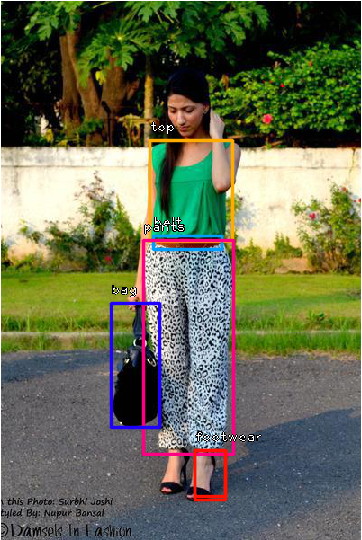
\includegraphics[width=.5\textwidth]{./figures/modanetfix/0892135_o} & 
		\includegraphics[width=.5\textwidth]{./figures/modanetfix/0892135_oc}\\
		
		%3rd row----------------------------
		\includegraphics[width=.5\textwidth]{./figures/modanetfix/0892135_} & 
		\includegraphics[width=.5\textwidth]{./figures/modanetfix/0892135_c}\\
		
	\end{tabular}
	\caption{Qualitative comparison of the ModaNet fix. On the first row, the original, on the second one, the fixed one. This is of course just one of many examples.}
	\label{f:modanet-fix} %% label for entire figure
\end{figure}
% --- figure ends --- % 

So here you can clearly see that the bounding boxes were overlapped before, and now they are correct. Even the polygons were wrong, and I corrected them. Not manually, but through a simple script that I'll describe more in detail below in \sref{s:fixing}.

What I want to point out here are what the elements are composed of. The bounding boxes are objects of 4 elements: the first is the top left corner of the box $x$ value, the second is the same, but the $y$ value, the third element is the width $\Delta x$, the fourth the height $\Delta y$.

Meanwhile for segmentation, each annotation is composed by different shapes that form a polygon. So let's say a shoe is, like our example, divided into two segments (that we call \emph{shapes}). The bottom shape and the top one together form the annotation that we can name “left shoe" if we desire. So, looking again at the structure in \sref{s:ds-modanet-struct}, we can specify that the \emph{polygon} is none other than a list of shapes.

My script recognized that the upper shape did not fit the right shoe and moved the shape to the left shoe's polygon.

A shape has also a simple structure. It's a list of points, like this: $[x1, y1, x2, y2,\dots]$
Those points form an enclosed shape, like a circle or a square (of course they are not as regular, it's just to make the point).

Therefore, those are the essential elements to start working on fixing the annotations, or even understanding how the annotations were fixed.

\section{A Python Package to automate the process}\label{s:ds-package}

As you can see in the Abstract at the beginning, I never did or even thought of doing a python package before, so I had to start from scratch. 

It was a very nice idea by Leonardo, though, because it allows for your months of work to be condensed into a small package that can be ready to train in just a few hours!

The \emph{Command Line Interface} (CLI) I was suggested to use is called \emph{Click} and, although I'd say not the most beautiful way of programming a CLI, it works quite well once you get the hang of it and make some modifications to your liking (just as I did). Another reminder that all my work is obviously published online on my GitHub (cad0p).

Initially this particular task was focused on one question: how do I automate the downloading process of the other repos? I can't just say: download ModaNet, put it there, download PaperDoll, put it there, and if you've done all of this then you can start using my program.

It must be a one click process. So I developed a function for my CLI that could download all of this:  \lstinline[language=bash]|maskrcnn-modanet datasets download /your/folder/here|

This function calls a bash script to download the necessary repos and creating the folder structure you see in \fref{f:datastructure}.

\begin{figure}[H]
	\centering
	\includegraphics[width=\linewidth]{figures/cli/main}
	\caption{The main CLI page of the package maskrcnn-modanet}
	\label{f:cli-main}
\end{figure}

\paragraph{savedvars}

I used a file located in the user's home folder/.maskrcnn-modanet to save the useful variables to keep in memory even after the program is closed. They ended up being just a few:

\begin{figure}[H]
	\centering
	\includegraphics[width=\linewidth]{figures/cli/savedvars}
	\caption{The saved variables of the package maskrcnn-modanet}
	\label{f:cli-savedvars}
\end{figure}

\paragraph{datasets}

Then I implemented the commands for the datasets, down here:

\begin{figure}[H]
	\centering
	\includegraphics[width=.75\linewidth]{figures/cli/datasets}
	\caption{The actions available to manage the datasets of the package maskrcnn-modanet}
	\label{f:cli-datasets}
\end{figure}

The ones I've already talked about, that I ported over the package, are to download the package and to arrange it (although arranging the dataset includes splitting the annotations too).

The fix one is the famous script described in \sref{s:ds-mn-fix}.

\emph{viewannotation} and \emph{viewimage} are programs completely related to the dataset, whatever they are fixed or not, so here they are described in detail:

\paragraph{viewannotation}

\begin{figure}[H]
	\centering
	\includegraphics[width=.75\linewidth]{figures/cli/viewannotation}
	\caption{The way to easily check out an annotation through the package maskrcnn-modanet}
	\label{f:cli-viewannotation}
\end{figure}

As you can see, you can provide the filename of the image you want to check out the annotations.
The original flag uses the original file (if the annotations have been fixed).
The parameter for a custom annotations file is mainly for testing purposes, to see if different fixes impact positively or negatively the quality of the annotations.

The end result is something like this:

\begin{lstlisting}[language=bash]
user@Delil:~/piercarlo$ maskrcnn-modanet viewannotation -p 0736791.jpg -o
\end{lstlisting}

\begin{lstlisting}[language=Python]
	[{'category_id': 2, 'iscrowd': 0, 'area': 1746, 'bbox': [160, 247, 97, 18], 'id': 0, 
	'segmentation': [[161, 248, 170, 248, 173, 249, 189, 251, 199, 252, 199, 250,...]], 'image_id': 736791}, 
	{'category_id': 4, 'iscrowd': 0, ....
	
\end{lstlisting}

\paragraph{viewimage}

\begin{figure}[H]
	\centering
	\includegraphics[width=.75\linewidth]{figures/cli/viewimage}
	\caption{The way to easily check out an annotated image through the package maskrcnn-modanet}
	\label{f:cli-viewimage}
\end{figure}

\emph{viewimage} is very useful to compare and see how the images are annotated. 
It's got the same options as the simpler \emph{viewannotation}, but some added ones worth mentioning and very useful are \lstinline[language=bash]|--all set| , \lstinline[language=bash]|--begin-from|, and \lstinline[language=bash]|--coco-way|.

\emph{all set} allows us to view multiple images without relaunching the command (and reloading 100MB of the annotations as a consequence) every time we want to see a new image.

\emph{begin from} works with all set by setting up a start point to view not only always the first images in the dataset and have a biased look at it.

\emph{coco way} uses the default coco library to show the annotations, and the end result is that, instead of showing the bboxes, it shows very beautifully the segmentation, coloring with a random color elements of the same annotation (polygon).

This is how the images in \fref{f:modanet-fix} were produced.

Those last two commands were the ones that showed me what was needed to fix the problem I oversaw for months.




\section{Datasets for competitions}\label{s:ds-cpt}

\subsection{ImageNet}\label{s:imagenet}
One of the greatest problems in AI has been in working with images and visual input. As we learned in \sref{s:cnn-structure}, convolutional neural networks are very effective at doing this. One of the great challenges that has pushed this field forward is ImageNet. ImageNet is a classification challenge where 1 million images are given and must be classified. Many groups all over the world strive to improve modern AI technology in order to top the charts annually. In order to produce more succesful results, many optimizations have been done to the standard neural network.

\subsubsection{Softmax}

The first challenge in this is how we can optimize determining which class something is. At the end of the network, we have one neuron per each output class (say 2 with dog and cat). We want to know which output class the image is. In simple cases, you can just take the highest. However, ImageNet allows you to take your top 5 best guesses since many classes turn out to be similar with thousands of classes (say different breeds of dogs). We want a way to estimate the probability of each label. To do this, we use the softmax layer, described in \sref{s:softmax}.

\subsubsection{VGG16}
\begin{figure}[H]
	\centering
	\includegraphics[scale=0.5]{images/vgg16}
	\caption{VGG16 Convolutional Network}
	\label{f:vgg16}
\end{figure}

One of the first networks that performed well combining all this so far was vgg16 \cite{pateria1990enhanced}. This network was able to classify images across thousands of categories with 90 percent accuracy given top 5 class guesses and 70.5 percent with top 1. This structure is still commonly used for many modern problems and has the benefits of being simple and easy to train. It has a slightly more powerful older cousin called vgg19 which is also very popular.
\subsubsection{ResNet}\label{s:imagenet-resnet}
\begin{figure}[H]
	\centering
	\includegraphics[width=0.65\textwidth]{images/resnetvsvgg}
	\caption{Resnet vs VGG19}
	\label{f:imagenet-resnet}
\end{figure}

For some years, the trend in machine learning was always adding more layers. With the constant improvement in GPUs, if something didn't work now, the solution was to wait a year and add more layers. However, one big issue that exists with this is the vanishing gradient. At some point, the connection between the input and the output is too spaced away and the network can no longer learn significant features at the lower layers. However, we know that deeper networks can learn more complex features more easily and are much better suited to handle hard problems. To solve this, researchers produced residual connections \cite{he2016deep}, which are described in \sref{s:blocks-resnet}.

As you can see, ResNet allows for much greater depth compared to VGG. This, too, is the smallest size of ResNet. Typical applications use ResNet-50 at least and high-end ones use ResNet-152. The sheer power of these structures has allowed for 92.9 percent accuracy on ImageNet and the usage of training on fancy GPUs with lots of data.

We indeed used ResNet-50 as backbone for our \maskrcnn.


\subsubsection{Inception}\label{s:imagenet-inception}
\begin{figure}[H]
	\centering
	\includegraphics[scale=0.5]{images/inception}
	\caption{Parallel Layers in Residual Note in Inception Neural Network.}
	\label{f:imagenet-inception}
\end{figure}

The last major improvement in recent years in image classification has been in the usage of multiple parallel layers in each residual node. Each of these sets of layers, as seen in the image above, contains different filter sizes, allowing for a varying size of features to be extracted. From this, each residual node can learn much more and increased information can be packed in. This has culminated in Inception-ResNet structures capable of producing results more accurate than humans on image classification.

Coincidentally, Tesla's neural network used for its Autonomous Driving features called “Autopilot", currently, as of V9 software (2019), still uses Inception V1.
\begin{quote}[teslamotorsclub.com]{jimmy-d}
	The V9 network takes 1280x960 images with 3 color channels and 2 frames per camera from, for example, the main camera. That’s 1280x960x3x2 as an input, or 7.3M. The V8 main camera was 640x416x2 or 0.5M - 13x less data.
\end{quote}

\subsubsection{To the Future}
In large part, following these advances, image classification has been solved. Without massive amounts of data, performance enhancements will largely be negligible. However, as these structures have gotten bigger, they have also gotten slower and slower. In recent years, the next step has been in breaking down multiple objects and analyzing complex images, as in \sref{s:nnevo}.

\subsection{COCO: Common Object in Context}\label{s:coco}
COCO is another popular dataset that handles further analysis in images. As the figure below shows, COCO images contain pixel level segmentation so that advanced structures like \maskrcnn and U-Nets can be trained. They also have 5 words associated with each image for image to text problems. There are approximately 200,000 annotated images.

The specific generator we're using is CocoGenerator. Generators introduced in \sref{s:img-gen}.

The \modanet annotations follow COCO's style too, considered standard for segmentation purposes.

\begin{center}
	\includegraphics[scale=0.45]{images/coco.PNG}
\end{center}

\subsection{PASCAL VOC}\label{s:voc}
This is another dataset similar to COCO that has pixel level segmentation. It has about 30,000 images and is older (2012).